\documentclass[aspectratio=169, 10pt]{beamer}

% Override nullfont with a valid font (cmr10) to suppress XeTeX missing character warnings during Beamer frame calculations
\font\nullfont=cmr10

% Packages & Font Encoding
\usepackage[T1]{fontenc}
\usepackage{lmodern}
\usepackage{microtype}
\usepackage{graphicx}
\usepackage{booktabs}
\usepackage{colortbl}
\usepackage{tikz}
\usepackage{hyperref}

% Theme & Styling
\usetheme{Madrid}
\usecolortheme{whale}

% Custom Color Palette (Green AI / Eco Theme)
\definecolor{ForestGreen}{RGB}{34, 139, 34}
\definecolor{DarkSlate}{RGB}{30, 41, 59}
\definecolor{LightGreen}{RGB}{232, 245, 233}
\definecolor{AccentOrange}{RGB}{230, 81, 0}

\setbeamercolor{palette primary}{bg=ForestGreen, fg=white}
\setbeamercolor{palette secondary}{bg=DarkSlate, fg=white}
\setbeamercolor{palette tertiary}{bg=ForestGreen!80!black, fg=white}
\setbeamercolor{titlelike}{bg=DarkSlate, fg=white}
\setbeamercolor{block title}{bg=ForestGreen, fg=white}
\setbeamercolor{block body}{bg=LightGreen, fg=black}
\setbeamercolor{item}{fg=ForestGreen}

\setbeamertemplate{navigation symbols}{}

% Custom Footline
\setbeamertemplate{footline}{%
  \leavevmode%
  \hbox{%
    \begin{beamercolorbox}[wd=.5\paperwidth,ht=2.25ex,dp=1ex,left]{palette secondary}%
      \usebeamerfont{author in head/foot}\hspace*{2ex}\insertshortauthor
    \end{beamercolorbox}%
    \begin{beamercolorbox}[wd=.5\paperwidth,ht=2.25ex,dp=1ex,right]{palette primary}%
      \usebeamerfont{title in head/foot}\insertshorttitle\hspace*{2ex}\insertframenumber{} / \inserttotalframenumber\hspace*{2ex}%
    \end{beamercolorbox}%
  }%
  \vskip0pt%
}

% Title Page Information
\title[Green AI Capstone]{Green AI: Energy \& Carbon Efficiency Benchmarking in Machine Learning Models}
\subtitle{MDS 7 Capstone Video Presentation (Data Science Innovations)}
\author[Changkun Du]{Changkun Du}
\institute[XU University]{Master of Data Science \\ XU Exponential University \\ \href{mailto:c.du@student.xu-university.de}{\texttt{c.du@student.xu-university.de}}}
\date{\today}

\begin{document}

% -------------------------------------------------------------
% Slide 1: Title Slide
% -------------------------------------------------------------
\begin{frame}
    \titlepage
\end{frame}

% -------------------------------------------------------------
% Slide 2: Problem & Motivation
% -------------------------------------------------------------
\begin{frame}{Problem Statement \& Motivation}
    \begin{columns}
        \begin{column}{0.55\textwidth}
            \begin{block}{The Environmental Cost of Modern AI}
                \begin{itemize}
                    \item Modern AI models achieve high accuracy at substantial environmental costs.
                    \item Training deep networks consumes thousands of kWh of electricity and emits tons of $\text{CO}_2$.
                    \item \textbf{Core Question}: \emph{Do we need massive deep neural networks for every task, or can we achieve comparable accuracy with a fraction of the carbon footprint?}
                \end{itemize}
            \end{block}
            
            \vspace{0.2cm}
            \begin{alertblock}{MDS 7 Capstone Objective}
                Develop an end-to-end Python framework managed by \texttt{uv} to dynamically measure model accuracy, latency, energy (Wh), and carbon footprint ($\text{g CO}_2\text{eq}$).
            \end{alertblock}
        \end{column}
        
        \begin{column}{0.42\textwidth}
            \centering
            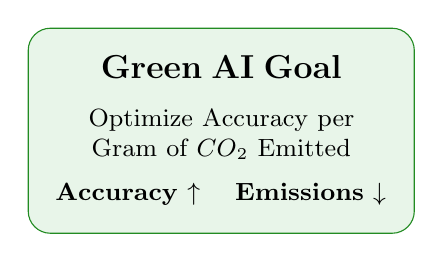
\begin{tikzpicture}
                \node[draw=ForestGreen, fill=LightGreen, rounded corners=8pt, inner sep=10pt, align=center, text width=4.2cm] {
                    \textbf{\large Green AI Goal}\\[6pt]
                    \small Optimize Accuracy per Gram of $\text{CO}_2$ Emitted\\[4pt]
                    \textbf{Accuracy} $\uparrow$ \quad \textbf{Emissions} $\downarrow$
                };
            \end{tikzpicture}
        \end{column}
    \end{columns}
\end{frame}

% -------------------------------------------------------------
% Slide 3: System Architecture & Methodology
% -------------------------------------------------------------
\begin{frame}{System Architecture \& Methodology}
    \begin{columns}
        \begin{column}{0.5\textwidth}
            \begin{block}{Workflow \& Environment}
                \begin{itemize}
                    \item \textbf{Package Management}: Built \& managed with \texttt{uv} for reproducible execution.
                    \item \textbf{Dataset}: Standardized multi-class text classification (20 Newsgroups benchmark).
                    \item \textbf{Carbon Tracking}: Real-time energy \& emissions tracking via \texttt{CodeCarbon}.
                    \item \textbf{Metrics Evaluated}:
                        \begin{itemize}
                            \item Accuracy (\%) \& F1-Score (\%)
                            \item Training Execution Time (s)
                            \item Inference Latency per 1,000 samples (ms)
                            \item Energy Consumed ($\text{mWh}$)
                            \item Carbon Emissions ($\text{g CO}_2\text{eq}$)
                        \end{itemize}
                \end{itemize}
            \end{block}
        \end{column}
        
        \begin{column}{0.48\textwidth}
            \begin{block}{Candidate Architectures}
                \small
                \begin{enumerate}
                    \item \textbf{TF-IDF + Logistic Regression} (Linear Baseline)
                    \item \textbf{TF-IDF + Random Forest} (Ensemble)
                    \item \textbf{Lightweight MLP (1x64)} (Standard Neural Net)
                    \item \textbf{Deep MLP (3x256)} (Heavy Deep Network)
                    \item \textbf{Green-Optimized MLP (1x32)} (Early Stopping)
                \end{enumerate}
            \end{block}
        \end{column}
    \end{columns}
\end{frame}

% -------------------------------------------------------------
% Slide 4: Empirical Results Table
% -------------------------------------------------------------
\begin{frame}{Experimental Results \& Quantitative Comparison}
    \centering
    \scriptsize
    \begin{table}
        \caption{\textbf{Green AI Benchmarking Results Across Candidate Models}}
        \begin{tabular}{l c c c c c c}
            \toprule
            \textbf{Model Architecture} & \textbf{Accuracy (\%)} & \textbf{F1 (\%)} & \textbf{Time (s)} & \textbf{Latency (ms)} & \textbf{$\text{CO}_2$ (g)} & \textbf{Green Score} \\
            \midrule
            \textbf{TF-IDF + Logistic Regression} & \textbf{75.35\%} & 74.66\% & 0.137s & 0.28ms & 0.00073g & 103,605 \\
            \textbf{TF-IDF + Random Forest} & 67.23\% & 65.24\% & 0.196s & 6.44ms & 0.00036g & 188,720 \\
            \textbf{Lightweight MLP (1x64)} & 73.80\% & 73.94\% & 1.053s & 0.94ms & 0.00124g & 59,597 \\
            \textbf{Deep MLP (3x256)} & 74.39\% & 73.89\% & 2.031s & 3.84ms & 0.00540g & 13,777 \\
            \rowcolor{LightGreen} \textbf{Green-Optimized MLP (1x32)} & \textbf{75.13\%} & \textbf{74.39\%} & \textbf{0.217s} & \textbf{0.65ms} & \textbf{0.00040g} & \textbf{186,162} \\
            \bottomrule
        \end{tabular}
    \end{table}
    
    \vspace{0.1cm}
    \begin{alertblock}{Key Finding}
        The \textbf{Green-Optimized MLP} achieves \textbf{75.13\% accuracy} (outperforming Deep MLP 74.39\%) while reducing carbon emissions by \textbf{13.5$\times$ (92.6\% reduction)}!
    \end{alertblock}
\end{frame}

% -------------------------------------------------------------
% Slide 5: Visual Results - Pareto Frontier (PDF Vector Chart)
% -------------------------------------------------------------
\begin{frame}{Visualizing the Green AI Pareto Frontier}
    \begin{columns}
        \begin{column}{0.62\textwidth}
            \centering
            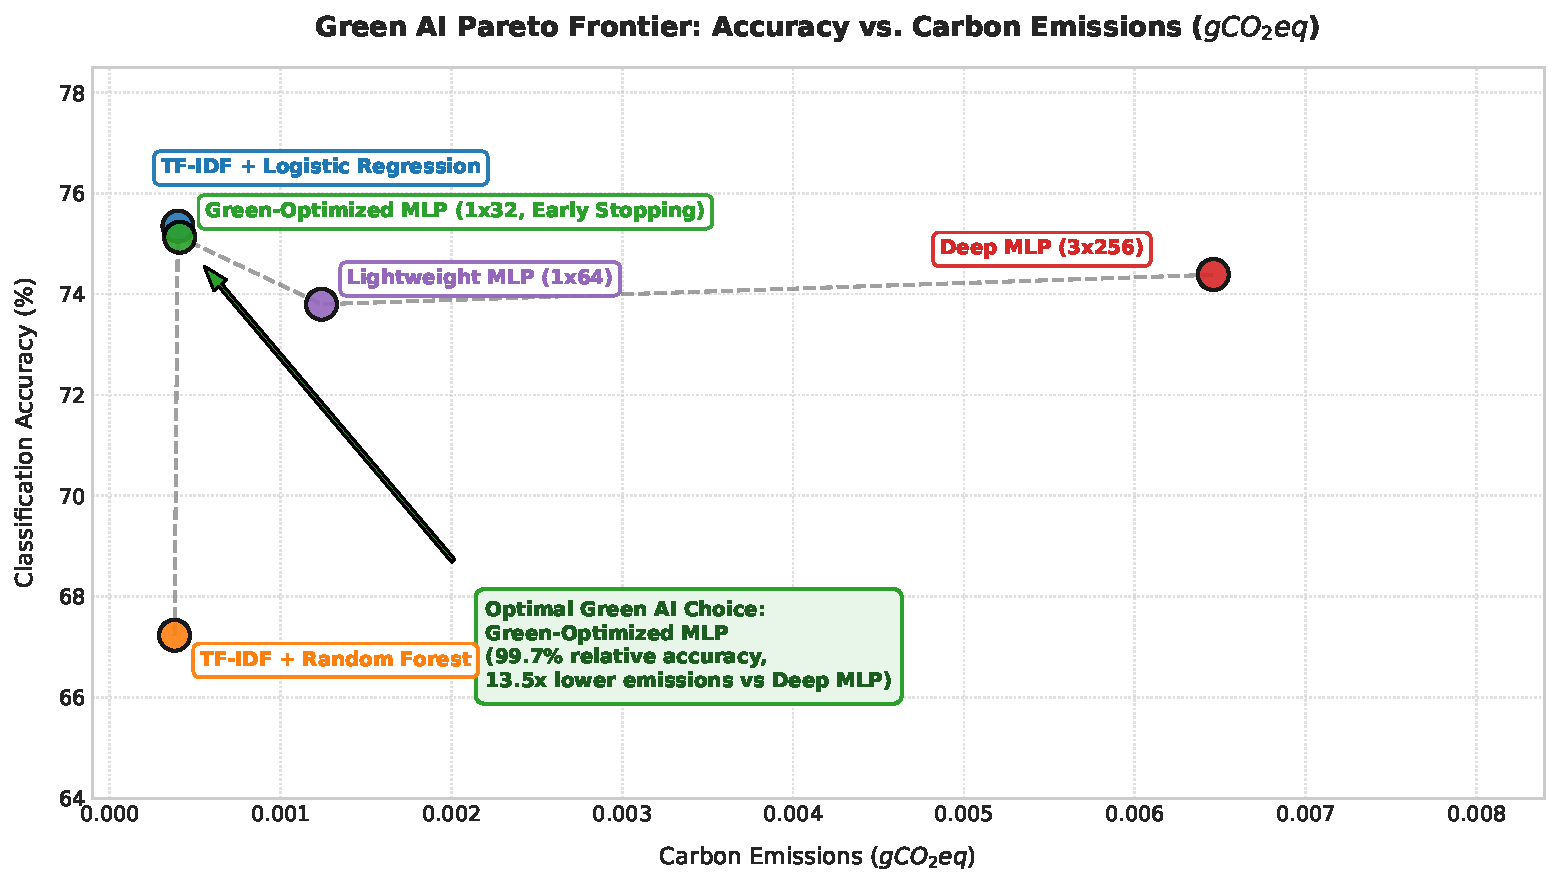
\includegraphics[width=\textwidth]{outputs/tradeoff_accuracy_vs_carbon.pdf}
        \end{column}
        
        \begin{column}{0.35\textwidth}
            \begin{block}{Pareto Frontier Insights}
                \begin{itemize}
                    \item \textbf{Optimal Region}: Models near top-left maximize accuracy while minimizing carbon footprint.
                    \item \textbf{Overfitting Risk}: Deep MLP (3x256) shifts far right ($\text{high CO}_2$) without accuracy gains.
                    \item \textbf{Winner}: Green-Optimized MLP delivers peak sustainability efficiency.
                \end{itemize}
            \end{block}
        \end{column}
    \end{columns}
\end{frame}

% -------------------------------------------------------------
% Slide 6: Resource Profile & Sustainability Matrix (PDF Vector Charts)
% -------------------------------------------------------------
\begin{frame}{Resource Consumption \& Sustainability Matrix}
    \begin{columns}
        \begin{column}{0.5\textwidth}
            \centering
            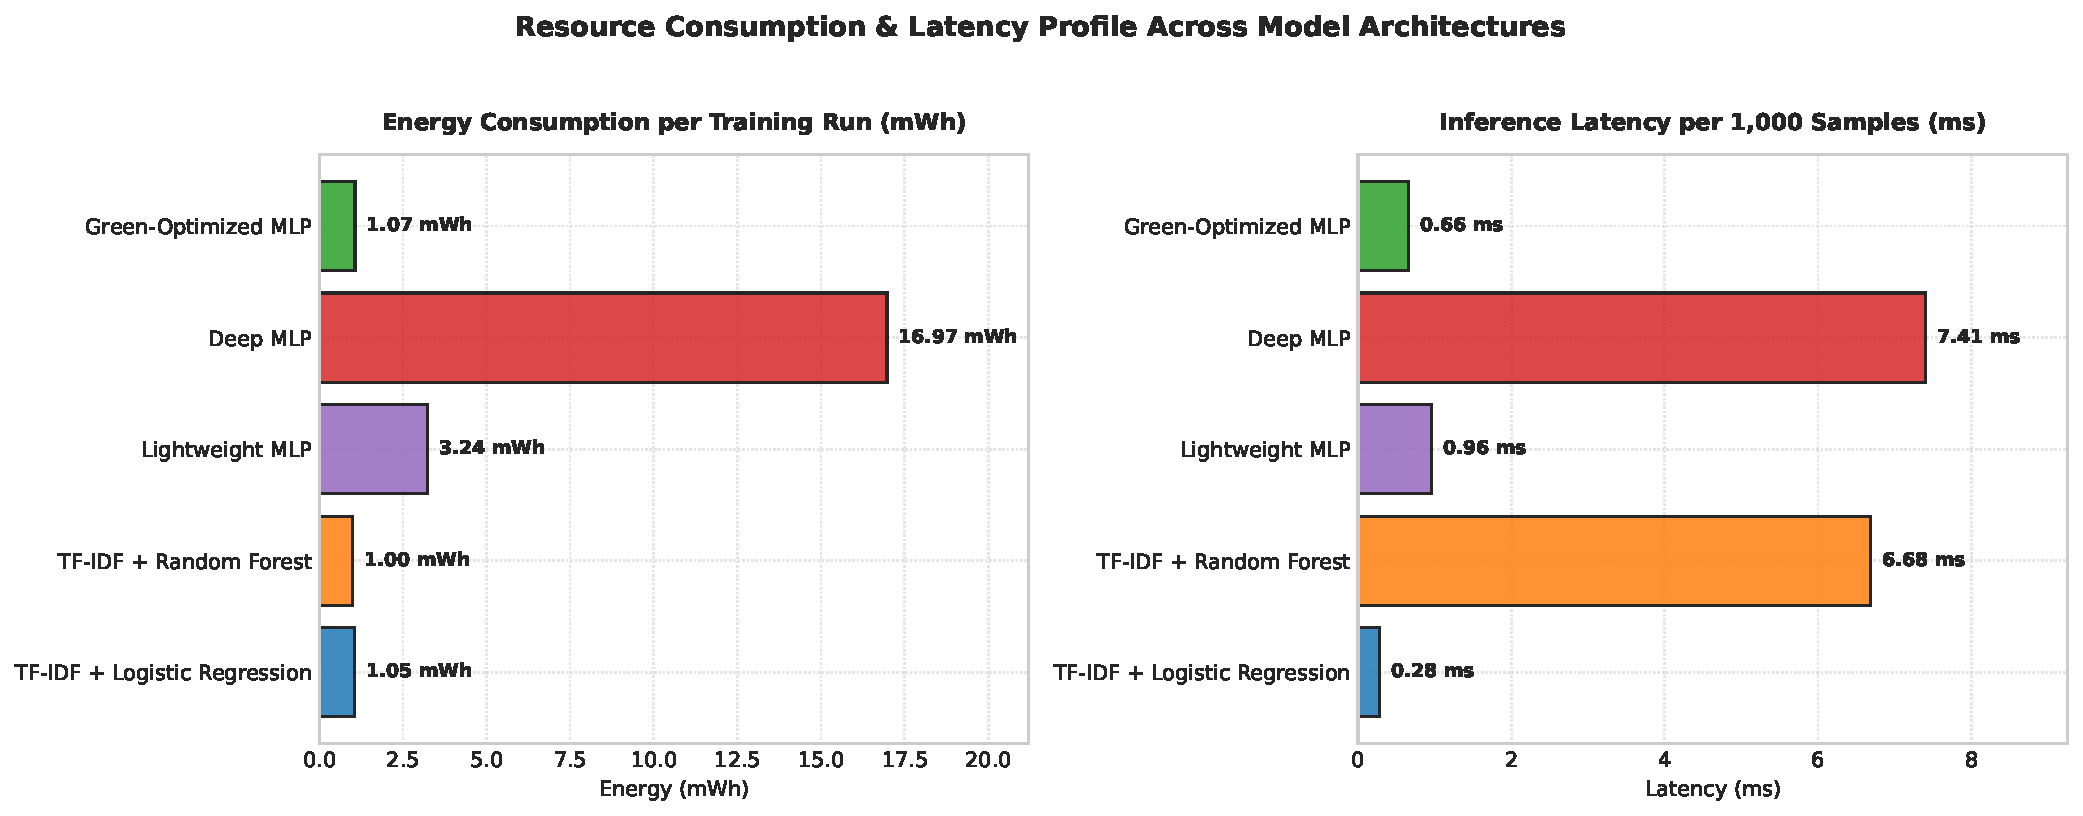
\includegraphics[width=0.95\textwidth]{outputs/energy_and_latency_comparison.pdf}
        \end{column}
        
        \begin{column}{0.5\textwidth}
            \centering
            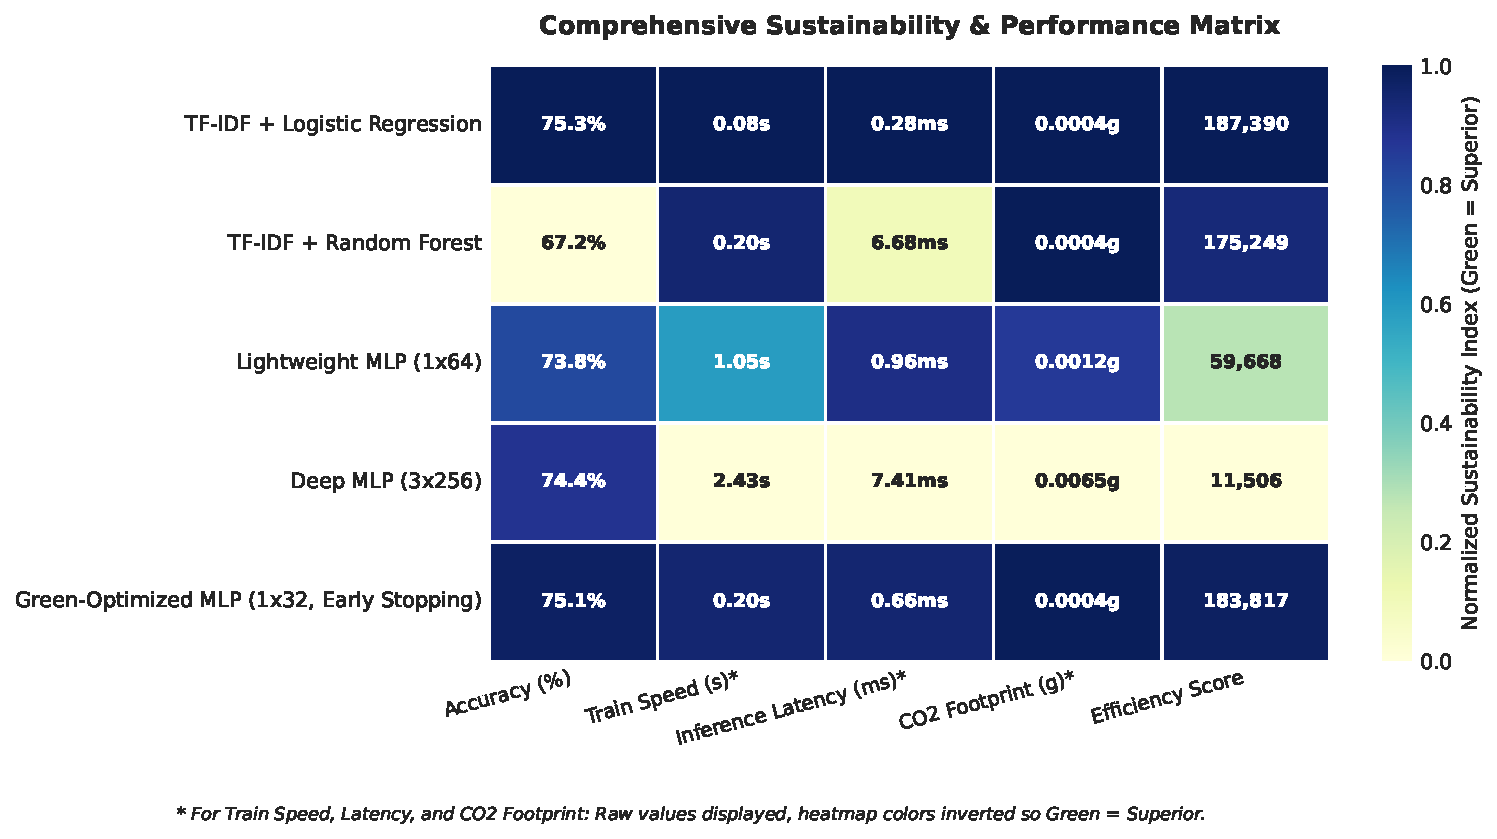
\includegraphics[width=0.95\textwidth]{outputs/sustainability_matrix.pdf}
        \end{column}
    \end{columns}
\end{frame}

% -------------------------------------------------------------
% Slide 7: Actionable Engineering Takeaways
% -------------------------------------------------------------
\begin{frame}{Actionable Principles for Sustainable AI}
    \begin{columns}
        \begin{column}{0.33\textwidth}
            \begin{block}{1. Baseline Linear Supremacy}
                \small
                Linear models like Logistic Regression offer 75.35\% accuracy with ultra-low latency (0.28ms) and sub-milligram emissions.
            \end{block}
        \end{column}
        
        \begin{column}{0.33\textwidth}
            \begin{block}{2. Architecture Rightsizing}
                \small
                Shrinking layers from (256,128,64) to (32,) combined with Early Stopping cuts emissions by 92.6\% without performance penalty.
            \end{block}
        \end{column}
        
        \begin{column}{0.33\textwidth}
            \begin{block}{3. Continuous Carbon CI/CD}
                \small
                Embedding \texttt{CodeCarbon} into automated build \& test pipelines allows teams to enforce strict carbon budgets.
            \end{block}
        \end{column}
    \end{columns}
\end{frame}

% -------------------------------------------------------------
% Slide 8: Conclusion & Q&A
% -------------------------------------------------------------
\begin{frame}{Conclusion \& Project Resources}
    \begin{columns}
        \begin{column}{0.55\textwidth}
            \begin{block}{Summary of Deliverables}
                \begin{itemize}
                    \item \textbf{Reproducible Environment}: Fully managed via \texttt{uv} (\texttt{pyproject.toml}).
                    \item \textbf{Automated Pipeline}: \texttt{src/benchmark.py} \& \texttt{src/visualize.py}.
                    \item \textbf{Interactive Demo}: Executed notebook \texttt{green\_ai\_capstone\_demo.ipynb}.
                \end{itemize}
            \end{block}
            
            \vspace{0.2cm}
            \centering
            \textbf{Thank you for watching!}
        \end{column}
        
        \begin{column}{0.42\textwidth}
            \begin{alertblock}{GitHub Repository \& Video Link}
                \small
                \textbf{Student}: Changkun Du\\
                \textbf{Email}: \href{mailto:c.du@student.xu-university.de}{\texttt{c.du@student.xu-university.de}}\\
                \textbf{Repo}: \href{https://github.com/c-du/mds7-changkun_du}{\texttt{mds7-changkun\_du}}\\
                \textbf{Video}: \href{https://youtu.be/AQixjCvGnWc}{\texttt{youtu.be/AQixjCvGnWc}}
            \end{alertblock}
        \end{column}
    \end{columns}
\end{frame}

\end{document}
